\subsection{Reglas del crecimiento tumoral}
\label{subsec-celldiv}
El conjunto de reglas que se define a lo largo de esta secci\'on se relaciona con el comportamiento de las c\'elulas cancer\'igenas que conforman una masa tumoral. Dicho comportamiento se define a partir de un grupo de suposiciones que determinan la naturaleza macrosc\'opica del tumor as\'i como las interacciones entre las c\'elulas cancer\'igenas y las c\'elulas normales del tejido. Como se expuso en las hip\'otesis I y II sobre la progresi\'on idealizada del desarrollo tumoral y las mutaciones de las c\'elulas cancer\'igenas respectivamente, el desarrollo del tumor se divide en las etapas avascular y vascular, donde en cada etapa se manifiestan determinados comportamientos caracter\'isticos relacionados con la expresi\'on de las mutaciones representativas del c\'ancer. 

En el presente modelo se reproduce el desarrollo de dos tipos de tumores: el tumor primario y los tumores secundarios o met\'astasis, entre los cuales existen un n\'umero de diferencias clave en cuanto a las c\'elulas cancer\'igenas que lo conforman, a su comportamiento y a la influencia de factores del entorno. Un tumor primario est\'a conformado por c\'elulas que de forma ideal van adquiriendo las distintas mutaciones caracter\'isticas del c\'ancer, seg\'un lo expresado en la hip\'otesis II. En cambio las c\'elulas que conforman un tumor secundario son c\'elulas que culminaron este proceso de acumulaci\'on de mutaciones en el tumor primario que les di\'o origen, y luego realizaron la met\'astasis y colonizaci\'on de la nueva localizaci\'on de forma satisfactoria. Por lo que se puede concluir que durante la etapa vascular un tumor primario y los tumores secundarios est\'an conformados por c\'elulas que presentan el mismo grado de mutaciones, causando que ambos tipos de tumores en esta etapa se comportan de igual forma. Luego se asume que no existe diferencias entre un tumor primario y uno secundario cuando est\'an en etapa vascular, y ambos son capaces de llevar a cabo la invasi\'on, la migraci\'on y la met\'astasis. Pero, seg\'un la hip\'otesis II, durante la etapa avascular un tumor primario cuenta solamente con las mutaciones relacionadas con el ciclo celular mientras que las micromet\'astasis, o tumores secundarios en etapa avascular, cuentan con todas las mutaciones caracter\'isticas del c\'ancer, por lo que su comportamiento es distinto. Este comportamiento se traduce en su capacidad de invadir los tejidos sanos del \'organo donde crecen y su capacidad de llevar a cabo la met\'astasis. A su vez, la invasi\'on de un tejido sano se traduce en la capacidad del tumor de desplazar a los distintos tipos de c\'elulas normales correspondientes con estos tejidos de su posici\'on, mediante las fuerzas expansivas causadas por el aumento de la concentraci\'on de c\'elulas cancer\'igenas en el interior del tumor o por su propia descendencia. 

El c\'ancer representado en el modelo se conoce como carcinoma y tiene su origen en las c\'elulas epiteliales que revisten los \'organos. Un tumor primario de este tipo se expande dentro del epitelio y hacia el lumen durante la etapa avascular. Es producto de la angiog\'enesis que ocurre la degradaci\'on de la membrana basal y los cambios en la matriz de interacci\'on intercelular, procesos que le permiten al tumor desplazar los tejidos de sost\'en o estroma. Por tanto, durante la etapa vascular, la expansi\'on del tumor ocurre en el epitelio y el lumen, pero tambi\'en gana la capacidad de invadir el estroma. En cambio, una micromet\'astasis comienza a inducir la angiog\'enesis desde el inicio, por lo que posee la capacidad de invadir los distintos tejidos sanos durante la etapa avascular. No obstante, aunque la micromet\'astasis posee todos los criterios caracter\'isticos del c\'ancer, no comienza a expresar los relacionados con la migraci\'on y la met\'astasis hasta la etapa vascular. Se debe se\~nalar que la invasi\'on de los tejidos de sost\'en de un tumor primario en etapa avascular no tiene que ocurrir exactamente en el momento que se comienza a desarrollar la angiog\'enesis, pero constituye el caso promedio. En cuanto a la influencia de factores externos, una micromet\'astasis puede ser eliminada del aut\'omata por dos causas fundamentales: su destrucci\'on por parte del sistema inmunitario o su incapacidad de sobrevivir en el entorno donde crece, donde ambos factores poseen una estrecha relaci\'on con la teor\'ia de la semilla y el sustrato expuesta en la secci\'on~\ref{subsec-meta}. Se asume que un tumor en etapa vascular, sea primario o secundario, no puede ser eliminado por el sistema inmunitario y que se adapt\'o satisfactoriamente al entorno donde se desarrolla. Con el objetivo de que el aut\'omata represente todo el ciclo vital del c\'ancer, un tumor primario durante la etapa avascular no puede ser eliminado por el sistema inmunitario y posee la capacidad de sobrevivir en su localizaci\'on inicial. Estas caracterizaciones se recogen en el cuadro comparativo~\ref{table-comparison} y el ciclo vital del c\'ancer representado en este modelo se muestra en la figura~\ref{fig-tumor-progresion}. 

\begin{table}[!ht]
\begin{center}
\scalebox{0.9}{\begin{tabular}{|c|c|c|c|c|} \hline
\emph{Caracter\'isticas} & \multicolumn{2}{|c|}{\emph{Tumor primario}} & \multicolumn{2}{|c|}{\emph{Tumor secundario}} \\\cline{2-5}
 & \emph{Avascular} & \emph{Vascular} & \emph{Avascular*} & \emph{Vascular} \\\hline
\emph{Invasi\'on}        & No   & S\'i & S\'i & S\'i \\ \hline
\emph{Migraci\'on}       & No   & S\'i & No   & S\'i \\ \hline
\emph{Met\'astasis }     & No   & S\'i & No   & S\'i \\ \hline
\emph{Supervivencia en el}   & Siempre & Siempre & Existe la    & Siempre     \\ 
\emph{entorno de desarrollo} &         &         & Probabilidad &    \\ \hline
\emph{Destrucci\'on por el}  & Nunca   & Nunca   & Existe la    & Nunca   \\ 
\emph{sistema inmunitario}   &         &         & Probabilidad &      \\ \hline
\end{tabular}}
%\scalebox{0.85}{\includegraphics{img/table-comparison.png}}
\end{center}\vspace*{-0.6cm}
\caption[Comparaci\'on entre los dos tipos de tumores representados tomando en cuenta sus caracter\'isticas durante ambas etapas de su desarrollo]{Comparaci\'on entre los dos tipos de tumores representados tomando en cuenta sus caracter\'isticas durante ambas etapas de su desarrollo. \emph{En el cuadro:} (*) Un tumor secundario en etapa avascular se corresponde con una micromet\'astasis.}
\label{table-comparison}
\end{table}

\begin{figure}[!ht]
\begin{center}
\scalebox{0.8}{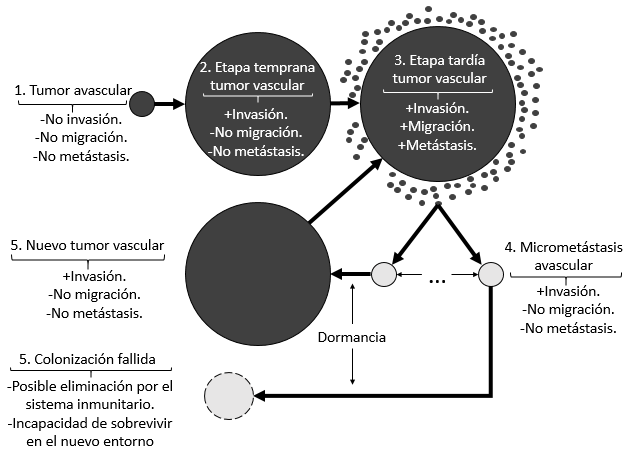
\includegraphics{img/fig-tumor-progresion-2.png}}
\end{center}\vspace*{-0.6cm}
\caption[Ciclo vital del c\'ancer representado por el modelo]{Ciclo vital del c\'ancer representado por el modelo. Como se puede apreciar la \'unica diferencia existente en el modelo entre un tumor primario y uno secundario es su comportamiento durante la etapa avascular, ya que se asume que un tumor primario siempre sobrevive y se desarrolla de forma satisfactoria en su entorno, mientras que una micromet\'astasis puede fallar en colonizar su nuevo entorno o ser destruida por el sistema inmunitario.}
\label{fig-tumor-progresion}
\end{figure}

En la presente secci\'on, referente al surgimiento de c\'elulas tumorales que conforman la masa neopl\'asica, se expone el procedimiento seguido para definir las reglas que reproducen el crecimiento de un tumor primario en ambas etapas y de los tumores secundarios durante la etapa vascular. La transici\'on entre las etapas avascular y vascular en un tumor primario ocurre de forma natural cuando su poblaci\'on celular alcanza cierto punto, mientras que en una met\'astasis esta transici\'on est\'a determinada por un proceso conocido como dormancia o latencia\footnote{De ahora en adelante cuando se utilice la palabra tumor nos estaremos refiriendo a un tumor primario o a un tumor secundario en etapa vascular, salvo que se especifique lo contrario.}. El crecimiento de un tumor secundario durante la etapa avascular y el proceso de dormancia ser\'an expuestas en las secciones~\ref{subsec-micrometastasis} y~\ref{subsec-dormancy}. 

Como se mostr\'o anteriormente la vascularizaci\'on de un tumor es un elemento distintivo de su desarrollo, ya que la difusi\'on de nutrientes permite al propio tumor crecer solo hasta un l\'imite permitido, y es el nuevo suministro de nutrientes proveniente de la neovasculatura la que permite que el tumor contin\'ue su crecimiento m\'as all\'a de dicho l\'imite. Como se mostr\'o en la hip\'otesis VIII sobre el desarrollo tumoral en funci\'on de la poblaci\'on, el modelo asume que la din\'amica de un tumor sigue la funci\'on de crecimiento log\'istico de Verhulst~\cite{verhulst}, presentada a continuaci\'on:
\begin{equation}
\left\lbrace
	\begin{array}{l}		
		\displaystyle\frac{dP}{dt} = rP(1-\displaystyle\frac{P}{K})\vspace*{0.2cm}\\
		P(t=0)=P_0
	\end{array}
\right., \label{eq-verhulst}
\end{equation}
donde se expresa que la variaci\'on de la poblaci\'on respecto al tiempo depende de un ritmo de crecimiento $r$, la poblaci\'on $P$ en ese instante de tiempo y un valor $K$ que representa la capacidad de carga, es decir, la cantidad de individuos de la poblaci\'on que puede sostener el entorno. La angiog\'enesis se puede traducir como un aumento de la capacidad de carga $K$ del entorno, as\'i como un incremento en el ritmo de proliferaci\'on celular debido a que la neovasculatura constituye un m\'etodo de suministro m\'as eficiente que la difusi\'on de nutrientes. Por tanto la din\'amica global del crecimiento ser\'a descrita por dos expresiones: una correspondiente con la etapa avascular y una correspondiente con la etapa vascular, ambas con sus par\'ametros particulares. Como consecuencia del an\'alisis anterior se adopta la siguiente hip\'otesis:

\begin{itemize}
\item [{XIV.}] \textbf{Interpretaci\'on de la neovasculatura}: \emph{Se asume que la neovasculatura que crece en el interior de un tumor producto de la angiog\'enesis produce un aumento en la capacidad de carga del entorno y en el ritmo de proliferaci\'on del propio tumor.} \label{XIV}
\end{itemize} 

En las reglas sobre la conservaci\'on del estado de las c\'elulas normales del aut\'omata~(\ref{eq-inert}) se especific\'o que dichas c\'elulas no cambian de estado salvo que en se encuentren en presencia de c\'elulas cancer\'igenas pertenecientes a alg\'un tumor. Esto significa que la regla del crecimiento tumoral se puede definir a partir de esta condici\'on, es decir, las c\'elulas normales tienen una probabilidad de ser desplazadas de su posici\'on si se encuentran pr\'oximas a una o varias c\'elulas cancer\'igenas pertenecientes a uno o distintos tumores, o en t\'erminos de la funci\'on~(\ref{eq-near-neighbours}) $\mathcal{N}_3^n(S(v,n)) > 0$. Por tanto las reglas se definen de la siguiente forma:
\begin{equation}
s(v,n+1)=\mathcal{R}(S(v,n))=\left\lbrace
	\begin{array}{ll}
		\zeta_0(S(v,n))& \textit{si } s(v,n)=0~\wedge~\mathcal{N}_3^n(S(v,n)) > 0 \\
		\zeta_1(S(v,n))& \textit{si } s(v,n)=1~\wedge~\mathcal{N}_3^n(S(v,n)) > 0 \\
		\zeta_2(S(v,n))& \textit{si } s(v,n)=2~\wedge~\mathcal{N}_3^n(S(v,n)) > 0 
	\end{array}
\right., \label{eq-celldiv}
\end{equation}
donde $\zeta_i(S(v,n)) \in \lbrace i,3 \rbrace$ con $i \in \lbrace 0,1,2 \rbrace$ son variables aleatorias con la siguiente distribuci\'on de probabilidad:
\begin{subequations}
\begin{equation}
P(\zeta_i(S(v,n))=i) = 1 - \rho(S(v,n) \rightarrow 3),
\end{equation}
\begin{equation}
P(\zeta_i(S(v,n))=3) = \rho(S(v,n) \rightarrow 3).
\end{equation}
\end{subequations}

De las expresiones anteriores se infiere que la probabilidad de que una c\'elula normal sea desplazada por una c\'elula cancer\'igena tiene el valor correspondiente con la evaluaci\'on de la probabilidad de transici\'on $\rho(S(v,n) \rightarrow 3)$, mientras que la probabilidad de que permanezca en el estado original es $1-\rho(S(v,n) \rightarrow 3)$. Como un tumor siempre se expande hacia posiciones vecinas ocupadas por c\'elulas normales se puede asegurar que la masa tumoral posee una forma compacta donde cada c\'elula cancer\'igena posee en su vecindad a otras c\'elulas cancer\'igenas, en correspondencia con lo expresado en la hip\'otesis X sobre la adhesi\'on celular. Esta probabilidad de transici\'on, seg\'un la concepci\'on cl\'asica de un aut\'omata celular, debe definirse de forma tal que utilice solamente la informaci\'on de la configuraci\'on local para estimar el valor resultante. En el contexto del presente modelo es necesario que la probabilidad incorpore la informaci\'on relacionada con el modelo de crecimiento log\'istico.

\subsubsection{Proceso de inferencia de la regla}
La concepci\'on cl\'asica de un aut\'omata celular plantea que la funci\'on de transici\'on local solo puede recibir como argumento la configuraci\'on local de la c\'elula $v$ elegida para su actualizaci\'on~\cite{book}. Esto representa una limitaci\'on del modelo cl\'asico ya que no permite reproducir un n\'umero de procesos biol\'ogicos, tecnol\'ogicos y sociales en los que las posibles transiciones dependen de informaci\'on adicional. Entre los posibles ejemplos se encuentra la modelaci\'on de procesos de crecimiento en los que el n\'umero total de individuos y el potencial de reproducci\'on de la especie constituyen factores que influyen positiva o negativamente en la din\'amica poblacional, y como consecuencia en su probabilidad de crecimiento. Ante esta problem\'atica la idea de varios investigadores~\cite{guinot,ruben,ruanxiaoca,ruanxiaodiff} ha sido proponer extensiones del modelo de aut\'omatas celulares para incluir informaci\'on adicional de alguna forma en la funci\'on de transici\'on local. 

En~\cite{guinot} se expone una metodolog\'ia para la inferencia de reglas estoc\'asticas de un aut\'omata celular a partir de modelos continuos. Esta metodolog\'ia nos presenta nociones que pueden ser utilizadas para extender la concepci\'on cl\'asica. En el presente modelo se combina la probabilidad de transici\'on con las diferentes configuraciones locales que pueden darse, es decir, el criterio de selecci\'on de la regla que se debe aplicar en cada caso depende del estado de la configuraci\'on local, mientras que la probabilidad de transici\'on se obtiene a partir del modelo continuo. La adopci\'on de estas ideas es especialmente favorable ya que la funci\'on de transici\'on local y el criterio de selecci\'on de la regla a aplicar se mantienen de acuerdo a la definici\'on cl\'asica, y solo se modifica la probabilidad de transici\'on. Los nuevos argumentos de la probabilidad de transici\'on constituyen dependencias heterog\'eneas de la funci\'on de transici\'on que no est\'an concebidas en la concepci\'on cl\'asica de los aut\'omatas celulares. Se comienza especificando una probabilidad de transici\'on alternativa que reciba la informaci\'on pertinente al modelo continuo~\cite{guinot}.

\begin{definition}
\label{prop-newlocal-func}
Sea una extensi\'on de la funci\'on de transici\'on local definida en~\ref{def-local-func} que incluye una probabilidad de transici\'on alternativa que depende de nuevos argumentos:
\begin{equation}
s(v,n+1) = \mathcal{R}(S(v,n)) = e_i~~\textit{con probabilidad } \rho(\tau(v,n,N_{tum}) \rightarrow e_i), \label{eq-newlocal-func}
\end{equation}
donde $\tau(v,n,N_{tum})$ es una funci\'on que devuelve el tiempo transcurrido relativo al surgimiento del tumor que intenta expandirse hacia $v$ en el instante de tiempo $n$; e.g. si el instante de tiempo en que surgi\'o el tumor en cuesti\'on es $n'$ el tiempo transcurrido relativo es $n_r = n - n'$. 
\end{definition}

El conjunto $N_{tum}$ contiene la informaci\'on correspondiente con los instantes de tiempo en que surgieron los tumores contenidos en la simulaci\'on. Con el objetivo de ilustrar de forma clara el proceso de inferencia se asume durante esta secci\'on que solo existe un tumor expandi\'endose hacia la c\'elula $v$. En la secci\'on que se muestra a continuaci\'on que trata sobre la inclusi\'on de nuevas hip\'otesis al modelo se esclarece esta suposici\'on exponiendo un m\'etodo de resoluci\'on de las distintas situaciones de competencia que pueden surgir entre varios tumores cuando se expanden hacia una misma c\'elula. En el algoritmo~\ref{alg-n-r} se muestra la implementaci\'on de la funci\'on $\tau(v,n,N_{tum})$ a modo de definici\'on donde se tiene en cuenta la suposici\'on hecha anteriormente, $N^n(v)$ es la funci\'on de vecindad inmediata definida en~\ref{def-neighbourhoods}, la funci\'on $tumor(w)$ devuelve el identificador \'unico asociado al tumor al que pertenece $w$ y la funci\'on $s(w,n)$ es el estado de la c\'elula $w$ en el instante de tiempo $n$ definida en~\ref{def-cellstatus}. Aunque funciones como $\tau(v,n,N_{tum})$ pueden ser definidas matem\'aticamente, se prefiere la definici\'on mediante un algoritmo pues brinda informaci\'on adicional sobre la implementaci\'on del aut\'omata celular.

\begin{algorithm}[!ht]
\caption{Definici\'on de la funci\'on $\tau(v,n,N_{tum})$.} \label{alg-n-r}
\KwData{$v, n, N_{tum}$}
\KwResult{$n_r$}
\For{$w \in N^n(v)$}{
	\If{$s(w,n)=3$}{
		$n_r = n - N_{tum}[tumor(w)]$\;
		\Return $n_r$\;}}
\end{algorithm}

Se reescribe la regla de la aparici\'on de c\'elulas tumorales~(\ref{eq-celldiv}) tomando en cuenta la nueva probabilidad de transici\'on alternativa propuesta en~(\ref{prop-newlocal-func}) como:
\begin{equation}
s(v,n+1)=\mathcal{R}(S(v,n))=\left\lbrace
	\begin{array}{ll}
		\zeta_0(\tau(v,n,N_{tum}))& \textit{si } s(v,n)=0~\wedge~\mathcal{N}_3^n(S(v,n)) > 0 \\
		\zeta_1(\tau(v,n,N_{tum}))& \textit{si } s(v,n)=1~\wedge~\mathcal{N}_3^n(S(v,n)) > 0 \\
		\zeta_2(\tau(v,n,N_{tum}))& \textit{si } s(v,n)=2~\wedge~\mathcal{N}_3^n(S(v,n)) > 0 
	\end{array}
\right., \label{eq-celldiv-2}
\end{equation}
donde la distribuci\'on de probabilidad de las variables aleatorias $\zeta_i(\tau(v,n,N_{tum})) \in \lbrace i,3 \rbrace$ con $i \in \lbrace 0,1,2 \rbrace$ quedar\'ia como:
\begin{subequations}
\begin{equation}
P(\zeta_i(\tau(v,n,N_{tum})=i) = 1 - \rho(\tau(v,n,N_{tum}) \rightarrow 3),
\end{equation}
\begin{equation}
P(\zeta_i(\tau(v,n,N_{tum})=3) = \rho(\tau(v,n,N_{tum}) \rightarrow 3).
\end{equation}
\end{subequations}

El c\'alculo de la probabilidad de transici\'on $\rho(\tau(v,n,N_{tum}) \rightarrow 3)$ se define a partir de la ecuaci\'on de crecimiento log\'istico de Verhulst. Primero se debe escribir la ecuaci\'on de crecimiento de forma tal que podamos expresar la variaci\'on de la poblaci\'on desde un instante de tiempo $n$ hacia el instante $n+1$. Para valores peque\~nos de $\Delta t$, la derivada de la ecuaci\'on de crecimiento se puede determinar de forma aproximada como: 
\begin{subequations}
\begin{equation}
\frac{dP(t)}{dt} \approx \frac{P(t+\Delta t) - P(t)}{\Delta t},
\end{equation}
\begin{equation}
P'(t) \approx \frac{P(t+\Delta t) - P(t)}{\Delta t},
\end{equation}
\begin{equation}
\Delta t P'(t) \approx P(t+\Delta t) - P(t),
\end{equation}
\begin{equation}
P(t+\Delta t) - P(t) \approx \Delta t P'(t),
\end{equation}
\end{subequations}
luego si tomamos el tiempo $t$ como una variable discreta, y hacemos $t=n\Delta t$, obtenemos:
\begin{subequations}
\begin{equation}
P(n\Delta +\Delta t) - P(n\Delta t) \approx \Delta t P'(n\Delta t),
\end{equation}
\begin{equation}
P((n+1)\Delta t) - P(n\Delta t) \approx \Delta t P'(n\Delta t). \label{eq-delta}
\end{equation}
\end{subequations}

La expresi\'on~(\ref{eq-delta}) se interpreta como la variaci\'on de la poblaci\'on del tumor entre los instantes de tiempo $n$ y $n+1$ como se puede apreciar en la parte izquierda $P((n+1)\Delta t) - P(n\Delta t)$. El tiempo que transcurre en el modelo continuo entre los instantes de tiempo $n$ y $n+1$ del aut\'omata celular es $\Delta t$. Se infiere de~(\ref{eq-delta}) que la probabilidad de transici\'on $\rho(\tau(v,n,N_{tum})\rightarrow 3)$ se calcula mediante $P'(t)$. A partir de~(\ref{eq-verhulst}), sujeta a la condici\'on inicial, se obtiene~(ver ap\'endice~\ref{app-a} para el proceso de resoluci\'on):
\begin{equation}
P(t) = \frac{P_0 K}{P_0 + (K-P_0)e^{-rt}}, \label{eq-verhulst-solution}
\end{equation} 
cuya derivada $P'(t)$ finalmente tiene la forma~(ver ap\'endice~\ref{app-b} para el proceso de derivaci\'on):
\begin{equation}
P'(t) = \frac{P_0 K r e^{rt}(K-P_0)}{(P_0 e^{rt} + K - P_0)^2}. \label{eq-prob}
\end{equation}

Se expuso anteriormente que la probabilidad de transici\'on $\rho(\tau(v,n,N_{tum}) \rightarrow 3) \in [0,1]$, lo cual no ocurre con la funci\'on $P'(t)$, por lo que es necesario analizar su imagen. Con este objetivo derivamos la funci\'on $P'(t)$ para buscar los puntos estacionarios~(ver ap\'endice~\ref{app-c} para el proceso de derivaci\'on), obteni\'endose: 
\begin{equation}
P''(t) = \frac{P_0 K r^2 e^{rt} (P_0-K)(P_0 e^{rt} + P_0 - K)}{(P_0 e^{rt} + K - P_0)^3},
\end{equation}
donde se infiere que $P'(t)$ posee un m\'aximo cuando:
\begin{equation}
t = \frac{1}{r} \ln\frac{K-P_0}{P_0}, \label{eq-cond-t}
\end{equation}
evaluando $P'(t)$ en este valor de $t$ obtenemos la probabilidad m\'axima de crecimiento:
\begin{equation}
P'\left(t = \frac{1}{r} \ln\frac{K-P_0}{P_0}\right) = \frac{Kr}{4}.
\end{equation}

Por tanto $P'(t)$ alcanza su valor m\'aximo en el punto $(\frac{1}{r} \ln\frac{K-P_0}{P_0}, \frac{Kr}{4})$, donde este valor depende directamente de la capacidad de carga $K$ y del ritmo de crecimiento $r$, devolviendo el intervalo de probabilidad $[0, \frac{Kr}{4}]$. Supongamos que $\rho_{max}$ es el valor m\'aximo de la funci\'on $P'(t)$ en su dominio, de tal forma que $P'(t) \in [0, \rho_{max}]$ sujeto a la condici\'on $\rho_{max} \leq 1$. Despejando la siguiente desigualdad:
\begin{equation}
\frac{K r}{4} \leq \rho_{max},
\end{equation}
se obtiene la condici\'on necesaria para que la funci\'on $P'(t) \in [0,\rho_{max}]$, quedando:
\begin{equation}
r \leq \frac{4 \rho_{max}}{K}. \label{eq-cond-1}
\end{equation}

Mediante la condici\'on~(\ref{eq-cond-1}) se puede asegurar que la probabilidad de crecimiento tumoral que se obtiene mediante la evaluaci\'on de $P'(t)$ pertenece al intervalo $[0,\rho_{max}]$, permitiendo un mecanismo de ajuste del modelo mediante la adecuada selecci\'on de $\rho_{max}$. Este mecanismo de ajuste se sustenta en el hecho de que los modelos de aut\'omatas que se recogen en trabajos anteriores se dividen en dos clases generales: los que reproducen un modelo concebido espec\'ificamente para la reproducci\'on del crecimiento de tumores como~\cite{ruben}, y los que reproducen un modelo general de crecimiento y lo adaptan al caso espec\'ifico del crecimiento de tumores como~\cite{kansal,kansal3,ruanxiaoca}, categor\'ia a la que pertenece el presente trabajo. En el segundo tipo de trabajos es com\'un encontrar este mecanismo en la forma de una probabilidad base como se aprecia en~\cite{kansal}. La condici\'on~\ref{eq-cond-1} est\'a expresada en base a $r$ dado que el valor de $\rho_{max}$ se selecciona a priori y $K$ se determina directamente a partir de la informaci\'on existente acerca del proceso de crecimiento de un tumor, mientras que el proceso de estimar $r$ carece de una metodolog\'ia por lo que es imprescindible poseer la mayor cantidad de informaci\'on acerca de su valor. Las estimaciones de estos valores se llevan a cabo en la secci\'on~\ref{sec-validation}.

A partir de las hip\'otesis VIII y XIV sobre el desarrollo tumoral en funci\'on de la poblaci\'on y la interpretaci\'on de la neovasculatura respectivamente, se infiere que el crecimiento de la poblaci\'on tumoral se describe mediante dos expresiones correspondientes a las etapas avascular y vascular, cada una con sus valores propios del ritmo de crecimiento $r$ y capacidad de carga $K$. Se puede deducir que ambas etapas poseen tambi\'en valores propios de poblaci\'on inicial $P_0$, donde la poblaci\'on inicial de la etapa vascular $P_0^v$ se corresponde con la capacidad de carga del entorno durante la etapa avascular $K_a$, es decir, $K_a = P_0^v$. An\'alogamente se pueden definir a priori valores de probabilidad m\'aximos $\rho_{max}$ para cada una de estas etapas. Finalmente las probabilidades de transici\'on, con $t=n\Delta t$, quedar\'ian como:
\begin{subequations}
\begin{equation}
\rho_a(n\Delta t) = \displaystyle\frac{P_0^a K_a r_a e^{r_a n\Delta t}(K_a-P_0^a)}{(P_0^a e^{r_a n\Delta t} + K_a - P_0^a)^2},
\label{eq-pa}
\end{equation}
\begin{equation}
\rho_v(n\Delta t) = \displaystyle\frac{P_0^v K_v r_v e^{r_v n\Delta t}(K_v-P_0^v)}{(P_0^v e^{r_v n\Delta t} + K_v - P_0^v)^2}.
\label{eq-pv}
\end{equation}
\end{subequations}

Utilizando las expresiones~(\ref{eq-pa},~\ref{eq-pv}) y diferenciando las etapas del desarrollo tumoral en base a un nuevo par\'ametro $n_a$ que indica el per\'iodo de tiempo que dura la etapa avascular, escribimos la probabilidad de transici\'on $\rho(\tau(v,n,N_{tum}) \rightarrow 3)$ como:
\begin{equation}
\rho(\tau(v,n,N_{tum}) \rightarrow 3) = \left\lbrace
	\begin{array}{ll}
		\rho_a(\tau(v,n,N_{tum}) \Delta t)& \textit{si } \tau(v,n,N_{tum}) \leq n_a \\
		\rho_v((\tau(v,n,N_{tum})-n_a) \Delta t)& \textit{si } \tau(v,n,N_{tum}) > n_a
	\end{array}
\right.. \label{eq-generaldivrule}
\end{equation}

N\'otese en la expresi\'on para el c\'alculo de $\rho_v$ que el tiempo que se utiliza como par\'ametro es el relativo al inicio de la etapa vascular, es decir, $\tau(v,n,N_{tum})-n_a$. La expresi\'on~(\ref{eq-generaldivrule}) se conoce como probabilidad de transici\'on general del crecimiento tumoral y se utiliza como base para la definici\'on de las probabilidades particulares para el desplazamiento de cada tipo de c\'elula normal del aut\'omata. En los segmentos siguientes se exponen las hip\'otesis del modelo que se relacionan con las direcciones de expansi\'on y el crecimiento del tumor hacia distintos tipos de tejidos.

\subsubsection{Inclusi\'on de nuevas hip\'otesis}
El uso de la probabilidad de transici\'on~(\ref{eq-generaldivrule}) en esta forma tiene dos inconvenientes. El primero es que solo tiene en cuenta un tumor expandi\'endose hacia la posici\'on de la c\'elula $v$ como hab\'iamos supuesto anteriormente. En varias circunstancias se pueden dar situaciones donde dos o varios tumores compiten por expandirse hacia una misma posici\'on, es decir, que una c\'elula normal posea en su vecindad inmediata varias c\'elulas cancer\'igenas pertenecientes a distintos tumores cuyas descendencias intentan ocupar la posici\'on de la c\'elula normal. Esta competencia tiene que ser reflejada de alguna forma en la regla del crecimiento tumoral. El segundo es que la probabilidad de transici\'on est\'a expresada solamente en funci\'on de $\rho_a(n\Delta t)$ y $\rho_v(n\Delta t)$ y no incorpora la influencia de otros factores en el crecimiento. Un ejemplo de estos factores es la direcci\'on de la expansi\'on. Se ha demostrado en varias investigaciones que un tumor tiende a crecer en direcci\'on de donde provienen los nutrientes~\cite{kansal3} lo que constituye un sesgo en la direcci\'on de la expansi\'on. Este \'ultimo hecho representa, adem\'as, un factor importante en la direcci\'on de la migraci\'on de las c\'elulas cancer\'igenas durante la cascada metast\'asica~\cite{kansal3}. Otro ejemplo es la velocidad de expansi\'on tumoral. Dada la configuraci\'on de vecindad utilizada las c\'elulas vecinas de una c\'elula central no se encuentran a la misma distancia. Si se toma que la velocidad m\'axima de expansi\'on tumoral representada en el modelo se corresponde con ocupar una celda del aut\'omata de un instante de tiempo al otro, esta velocidad no puede ser la misma si la expansi\'on proviene de una c\'elula vecina a una distancia menor que si proviniese desde una c\'elula vecina a una distancia mayor. Esta situaci\'on se representa en la figura~\ref{fig-expansion-velocity}. La regla general del crecimiento tumoral no toma en cuenta estos factores, por lo que es necesaria su inclusi\'on. Comenzamos planteando las siguientes hip\'otesis del modelo:
\begin{figure}[!ht]
\begin{center}
\scalebox{0.45}{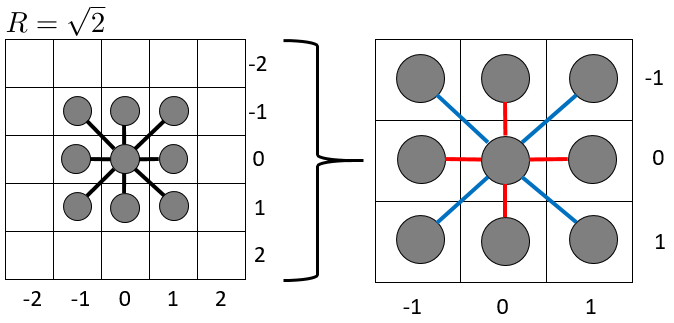
\includegraphics{img/fig-expansion-velocity.png}}
\end{center}\vspace*{-0.6cm}
\caption[Representaci\'on de las distintas velocidades de expansi\'on representadas en el modelo seg\'un la configuraci\'on de vecindad utilizada]{Representaci\'on de las distintas velocidades de expansi\'on representadas en el modelo seg\'un la configuraci\'on de vecindad utilizada. Las l\'ineas rojas en el diagrama derecho indican una mayor velocidad de expansi\'on que las l\'ineas azules. Esta noci\'on de velocidad se basa en la distancia entre estas c\'elulas.}
\label{fig-expansion-velocity}
\end{figure}

\begin{itemize}
\item [{XV.}] \textbf{Situaciones de competencia tumorales}: \emph{En las situaciones de competencia de varios tumores por expandirse a una misma posici\'on se asume que el valor de la probabilidad de transici\'on se corresponde con el tumor con mayor probabilidad de expansi\'on en ese momento. Si el tumor finalmente se expande hacia dicha posici\'on de forma satisfactoria, la nueva c\'elula cancer\'igena pertenece a dicho tumor.} \label{XV}

\item [{XVI.}] \textbf{Vectores de concentraci\'on de nutrientes}: \emph{Se asume que la concentraci\'on de nutrientes aumenta a medida que nos aproximamos a los tejidos de sost\'en y a la vasculatura del organismo. Este hecho se representa mediante uno o varios vectores en los \'organos del conjunto de c\'elulas del aut\'omata que indica las direcciones en que aumenta la concentraci\'on de los nutrientes.} \label{XVI}

\item [{XVII.}] \textbf{Sesgo direccional del crecimiento tumoral}: \emph{Se asume que la probabilidad de que aumente la poblaci\'on celular de un tumor se ve afectada por la concentraci\'on de los nutrientes. Este hecho constituye un sesgo en la direcci\'on del crecimiento del tumor, que se traduce en la tendencia a expandirse hacia la mayor concentraci\'on.} \label{XVII}

\item [XVIII.] \textbf{Velocidad de expansi\'on tumoral:} \emph{Se asume que la velocidad de expansi\'on tumoral depende de la distancia entre las c\'elulas tumorales y la c\'elula sana que intentan desplazar, que disminuye a medida que aumenta la distancia.} \label{XVIII}
\end{itemize}

Debe aclararse que la hip\'otesis XV tiene su fundamento biol\'ogico en que las cercan\'ias de una neoplasia con cierto grado de desarrollo la concentraci\'on de nutrientes es menor que en un tejido sano pues la masa tumoral consume una parte importante de los mismos. Luego cualquier tumor con un desarrollo inferior, en especial uno que posee un bajo grado o nulo de vascularizaci\'on, no tiende a expandirse hacia un tumor mayor que acapara la mayor parte de los nutrientes provenientes de la difusi\'on. Esta suposici\'on se refuerza con la hip\'otesis XVII y con la naturaleza oportunista y autorregulada del crecimiento tumoral. La hip\'otesis XVII permite explicar la expansi\'on del tumor en las distintas capas de tejidos que conforman los \'organos. Los tumores s\'olidos tienden a penetrar el estroma en busca de estos nutrientes a pesar de que presentan una mayor densidad, raz\'on por la que apenas crecen hacia el lumen del \'organo aunque presente una densidad nula. Con el objetivo de representar estas nuevas hip\'otesis del modelo es necesario reescribir la definici\'on de la probabilidad de transici\'on alternativa~(\ref{prop-newlocal-func}) como se muestra a continuaci\'on:

\begin{definition}
\label{prop-newlocal-func-2}
La funci\'on de transici\'on local definida en~\ref{prop-newlocal-func} se reescribe obteni\'endose una probabilidad de transici\'on alternativa que depende de nuevos argumentos:
\begin{equation}
s(v,n+1) = \mathcal{R}(S(v,n)) = e_i~~\textit{con probabilidad } \rho(\tau(v,n,N_{tum}) \rightarrow e_i), \label{eq-newlocal-func-2}
\end{equation}
donde $\tau(v,n,N_{tum})$ es una funci\'on que devuelve el conjunto de todos los tiempos transcurridos relativos al surgimiento de los tumores que intentan expandirse hacia $v$ en el instante de tiempo $n$; e.g. si los instantes de tiempo en que surgieron los tumores en cuesti\'on conforman el conjunto $\lbrace n_1', n_2', \ldots, n_m' \rbrace$ con $m$ la cantidad de tumores, el conjunto de tiempos transcurridos relativos es $n_r = \lbrace n-n_1',n-n_2', \ldots, n-n_m' \rbrace$.
\end{definition}

En el algoritmo~\ref{alg-n-r-2} se muestra la implementaci\'on de la nueva funci\'on $\tau(v,n,N_{tum})$ a modo de definici\'on donde se tiene en cuenta la hip\'otesis XV sobre las situaciones de competencia tumorales, $N^n(v)$ es la funci\'on de vecindad inmediata definida en~\ref{def-neighbourhoods}, la funci\'on $tumor(w)$ devuelve el identificador \'unico asociado al tumor al que pertenece $w$ y la funci\'on $s(w,n)$ es el estado de la c\'elula $w$ en el instante de tiempo $n$ definida en~\ref{def-cellstatus}. Se reescribe la regla del crecimiento tumoral~(\ref{eq-celldiv-2}) tomando en cuenta la nueva probabilidad de transici\'on alternativa~(\ref{eq-newlocal-func-2}) como:
\begin{equation}
s(v,n+1)=\mathcal{R}(S(v,n))=\left\lbrace
	\begin{array}{ll}
		\zeta_0(\tau(v,n,N_{tum}))& \textit{si } s(v,n)=0~\wedge~\mathcal{N}_3^n(S(v,n)) > 0 \\
		\zeta_1(\tau(v,n,N_{tum}))& \textit{si } s(v,n)=1~\wedge~\mathcal{N}_3^n(S(v,n)) > 0 \\
		\zeta_2(\tau(v,n,N_{tum}))& \textit{si } s(v,n)=2~\wedge~\mathcal{N}_3^n(S(v,n)) > 0 
	\end{array}
\right., \label{eq-celldiv-3}
\end{equation}
donde la distribuci\'on de probabilidad de las variables aleatorias $\zeta_i(\tau(v,n,N_{tum})) \in \lbrace i,3 \rbrace$ con $i \in \lbrace 0,1,2 \rbrace$ quedar\'ia como:
\begin{subequations}
\begin{equation}
P(\zeta_i(\tau(v,n,N_{tum}))=i) = 1 - \rho(\tau(v,n,N_{tum}) \rightarrow 3),
\end{equation}
\begin{equation}
P(\zeta_i(\tau(v,n,N_{tum}))=3) = \rho(\tau(v,n,N_{tum}) \rightarrow 3).
\end{equation}
\end{subequations}

\begin{algorithm}[t]
\caption{Definici\'on de la funci\'on $\tau(v,n,N_{tum})$.} \label{alg-n-r-2}
\KwData{$v, n, N_{tum}$}
\KwResult{$n_r$}
$n_r = \lbrace \rbrace$\;
\For{$w \in N^n(v)$}{
	\If{$s(w,n)=3$}{
		$n' = n - N_{tum}[tumor(w)]$\;
		$n_r = n_r \cup \lbrace n' \rbrace$\;}}
\Return $n_r$\;
\end{algorithm}

De acuerdo a la hip\'otesis XV sobre situaciones de competencia tumorales, la probabilidad de transici\'on~(\ref{eq-generaldivrule}) debe depender de las probabilidades de expansi\'on de cada uno de los tumores cuyos tiempos transcurridos relativos se encuentran en $\tau(v,n,N_{tum})$. Como se adopta la norma general que solo se expande el tumor con mayores posibilidades esta probabilidad de transici\'on puede ser escrita, tomando en cuenta la definici\'on~(\ref{prop-newlocal-func-2}), como:
\begin{equation}
\rho(\tau(v,n,N_{tum}) \rightarrow 3) = max\left[\rho(n_1 \rightarrow 3),\rho(n_2 \rightarrow 3),\ldots, \rho(n_m \rightarrow 3)\right], \label{eq-generaldivrule-2}
\end{equation}
donde $n_i \in \tau(v,n,N_{tum})$ con $i \in \lbrace 1,2,\ldots,m \rbrace$ y $m=|\tau(v,n,N_{tum})|$. La funci\'on $\rho(n_i \rightarrow 3)$ es la aplicaci\'on individual de la probabilidad de transici\'on a cada tumor contenido en el conjunto devuelto por la funci\'on $\tau(v,n,N_{tum})$. Se puede apreciar que el valor de la probabilidad de transici\'on global se corresponde con el m\'aximo de las probabilidades de expansi\'on de cada uno de los tumores que compiten por la posici\'on de la c\'elula $v$. La aplicaci\'on particular se escribe a partir de la probabilidad de transici\'on general del crecimiento tumoral~(\ref{eq-generaldivrule}):
\begin{equation}
\rho(n_i \rightarrow 3) = \left\lbrace
	\begin{array}{ll}
		\rho_a(n_i \Delta t)& \textit{si } n_i \leq n_a \\
		\rho_v((n_i - n_a) \Delta t)& \textit{si } n_i > n_a
	\end{array}
\right.. \label{eq-generaldivrule-3}
\end{equation}

Continuando con el proceso de incorporaci\'on de nuevas hip\'otesis a la probabilidad de transici\'on general del crecimiento tumoral, la hip\'otesis XVII sobre el sesgo direccional del crecimiento tumoral indica que la expansi\'on de un tumor tiende a producirse hacia una mayor concentraci\'on de nutrientes. Con el objetivo de simular la variaci\'on de dicha concentraci\'on en el tejido y tomando en cuenta la hip\'otesis XVI sobre los vectores de concentraci\'on de nutrientes se plantean las siguientes definiciones:

\begin{definition}
\label{def-regions}
Una regi\'on se define como:
\begin{equation}
R_i = \lbrace v~|~v \in V(G) : (x_{min} \leq v_x < x_{max})~\wedge~(y_{min} \leq v_y < y_{max}) \rbrace,
\end{equation}
donde $x_{min}$ y $y_{min}$ son los valores extremos inferiores de la regi\'on definida, mientras que $x_{max}$ y $y_{max}$ son los valores extremos superiores de la regi\'on definida. Las regiones definidas constituyen una partici\'on del conjunto de v\'ertices del grafo $V(G)$.
\end{definition}

\begin{definition}
\label{def-concentration}
Un vector de concentraci\'on expresa una direcci\'on hacia la cual aumenta el valor de la disponibilidad de nutrientes, tomando como regla general que el aumento ocurre en direcci\'on a los tejidos de sost\'en y a su vasculatura. Para simular condiciones heterog\'eneas en el interior de los \'organos cada uno de estos vectores est\'a asociado a una y solo una regi\'on dentro del mismo. El conjunto de vectores de concentraci\'on se denota como $B$, donde $B_i$ es el conjunto de vectores asociados al \'organo $i$ y $B_{ij}$ es el conjunto de vectores asociados al \'organo $i$ y a la regi\'on $R_j$ que pertenece a ese \'organo. 
\end{definition}

Por ejemplo en los diagramas izquierdo y centro de los cortes de tejidos mostrados en la figura~\ref{fig-structure} correspondientes con el aparato digestivo y las v\'ias a\'ereas inferiores del sistema respiratorio la variaci\'on de la concentraci\'on de nutrientes se puede representar mediante un vector que parte desde el tejido epitelial y apunta perpendicularmente hacia el estroma. En el caso del diagrama derecho de la figura~\ref{fig-structure} correspondiente con el h\'igado no hay necesidad de representar ning\'un vector ya que la vasculatura est\'a presente de manera uniforme en el \'organo haciendo de la concentraci\'on de nutrientes una magnitud homog\'enea. 

Generalmente se utiliza la similitud coseno para determinar el grado de similitud existente entre dos vectores mediante el valor del coseno del menor \'angulo comprendido entre ellos. En el presente trabajo se eval\'uan las similitudes coseno entre todos los vectores del conjunto $B$ que pertenecen a la regi\'on donde se localiza el tumor y el vector formado entre el centroide del tumor y la c\'elula $v$ hacia el que se est\'a expandiendo, tomando la mayor similitud como medida. Se interpreta esta medida como un coeficiente de las probabilidades de transici\'on de cada etapa del tumor $\rho_a(n \Delta t)$ y $\rho_v(n \Delta t)$, de manera el crecimiento se ve sesgado hacia la mayor concentraci\'on de nutrientes. A partir de lo expuesto anteriormente se plantean las siguientes definiciones:

\begin{definition}
\label{def-general-vector}
Sean dos c\'elulas $v$ y $w$ del conjunto $V(G)$. Un vector $\overrightarrow{\nu_{vw}}$ entre las c\'elulas $v$ y $w$ se define como:
\begin{equation}
\overrightarrow{\nu_{vw}} = \left(v_x - w_x, v_y - w_y \right). \label{eq-general-vector}
\end{equation}
\end{definition}

\begin{definition}
\label{def-sim}
Sean dos vectores $\overrightarrow{\nu_1}$ y $\overrightarrow{\nu_2}$, se define la similitud coseno $\beta(\overrightarrow{\nu_1},\overrightarrow{\nu_2})$ como el coseno del menor \'angulo, denotado como $\alpha$, comprendido entre ellos y se determina como:
\begin{equation}
\beta(\overrightarrow{\nu_1},\overrightarrow{\nu_2}) = \cos \alpha = \displaystyle\frac{\overrightarrow{\nu_1} \cdot \overrightarrow{\nu_2}}{|\overrightarrow{\nu_1}| \times |\overrightarrow{\nu_2}|}. \label{eq-sim}
\end{equation}
Como siempre toma el menor \'angulo comprendido entre los vectores, el mayor \'angulo comprendido posible es $\pi$ donde la similitud toma valor $-1$, que es el caso donde ambos vectores tienen direcciones opuestas. El menor \'angulo comprendido es $0$ donde la similitud toma valor $1$, correspondiente con el caso donde ambos vectores apuntan hacia la misma direcci\'on. La similitud toma valor $0$ cuando el \'angulo es $\pi /2$. Luego los valores posibles de la similitud coseno son:
\begin{equation}
\beta(\overrightarrow{\nu_1},\overrightarrow{\nu_2}) = \cos \alpha \in \left\lbrace
	\begin{array}{ll}
		\left[0,~1\right]& \textit{si } \alpha \in \left[0,\frac{\pi}{2} \right)\\
		\left[\textit{-}1,0\right]& \textit{si } \alpha \in \left[\frac{\pi}{2}, \pi \right]
	\end{array}
\right..
\end{equation}
\end{definition}

Como podemos apreciar, el valor de la similitud oscila entre $-1$ y $1$. La interpretaci\'on de los valores negativos puede ser inadecuada al ser utilizados como un coeficiente de probabilidad. Con el objetivo de penalizar el crecimiento tumoral contrario a los vectores de concentraci\'on de nutrientes y favorecerlo cuando dicho crecimiento ocurre en la misma direcci\'on se opta por utilizar una aplicaci\'on lineal que transforme el intervalo $[-1,1]$ de los valores de la similitud en el intervalo $[0$.$5, 1$.$5]$. De esta forma se penaliza la probabilidad de expansi\'on al multiplicarse por $0$.$5$ si este crecimiento es contrario a la direcci\'on indicada por los vectores de concentraci\'on, o se favorece al multiplicarse por $1$.$5$ si ocurre en la misma direcci\'on que la indicada por los vectores de concentraci\'on. De esta forma se mantiene el balance del crecimiento tumoral. En caso de que una probabilidad tome un valor mayor que $1$ al ser multiplicado por alg\'un coeficiente definido en el presente modelo su valor se hace igual a $1$. Se debe aclarar que si se toma el valor $0$ como penalizaci\'on del crecimiento tumoral negar\'ia la posibilidad de expansi\'on contraria a la direcci\'on indicada por los vectores de concentraci\'on de nutrientes. Esta nueva similitud alternativa se define a continuaci\'on:

\begin{definition}
\label{def-simprima}
Sean dos vectores $\overrightarrow{\nu_1}$ y $\overrightarrow{\nu_2}$, se define la similitud coseno alternativa $\beta_{alt}(\overrightarrow{\nu_1},\overrightarrow{\nu_2})$ como:
\begin{equation}
\beta_{alt}(\overrightarrow{\nu_1},\overrightarrow{\nu_2}) = \frac{1}{2} \beta(\overrightarrow{\nu_1},\overrightarrow{\nu_2}) + 1. \label{eq-simprima}
\end{equation}
La similitud coseno alternativa $\beta_{alt}(\overrightarrow{\nu_1},\overrightarrow{\nu_2}) \in [0$.$5, 1$.$5]$ cuando $\beta(\overrightarrow{\nu_1},\overrightarrow{\nu_2}) \in [-1, 1]$. 
\end{definition}

A partir de la expresi\'on~\ref{eq-simprima} se declara el coeficiente de la probabilidad de transici\'on $\beta_{tum}(v,l)$ como se muestra a continuaci\'on:

\begin{definition}
\label{def-beta}
La funci\'on $\beta_{tum}(v,l)$, que recibe una c\'elula $v$ y un tumor $l$, devuelve la m\'axima similitud coseno alternativa entre el vector $\overrightarrow{\nu_{vl}}$ y cada uno de los vectores de concentraci\'on del conjunto $B$ que pertenecen al mismo \'organo que el tumor $l$, es decir:
\begin{equation}
\beta_{tum}(v,l) = max\left[\beta_{alt}(\overrightarrow{b_{ij1}},\overrightarrow{\nu_{vl}}),\,\beta_{alt}(\overrightarrow{b_{ij2}}, \overrightarrow{\nu_{vl}})\,,\ldots,\,\beta_{alt}(\overrightarrow{b_{ijm}}, \overrightarrow{\nu_{vl}})\right], \label{eq-beta}
\end{equation}
donde $\overrightarrow{b_{ijk}} \in B_{ij}$ con $k \in \lbrace 1,2,\cdots,m \rbrace$ y $m=|B_{ij}|$ son los vectores de concentraci\'on asociados a la regi\'on $R_j$ del \'organo $i$ a la que pertenece la c\'elula $v$, o sea, $v \in R_j$, y $\overrightarrow{\nu_{vl}}$ es el vector formado por el c\'elula $v$ y el centroide del tumor $l$, donde el centroide constituye el punto de aplicaci\'on y $v$ el extremo del vector. 
\end{definition}

Las definiciones de un vector de expansi\'on y del centroide del tumor se presentan a continuaci\'on:

\begin{definition}
\label{def-centroid}
Sea $l=\lbrace w_1,w_2,\ldots,w_{m}\rbrace$ con $m=|l|$ un conjunto que contiene las c\'elulas pertenecientes a un tumor cualquiera representado en el aut\'omata. El centroide de dicho tumor se denota como $c_l$ y se define como el promedio de las componentes de las c\'elulas del conjunto, es decir:
\begin{equation}
c_l = \left(\frac{w_{1x} + w_{2x} + \ldots + w_{mx}}{m}, \frac{w_{1y} + w_{2y} + \ldots + w_{my}}{m} \right). \label{eq-centroid}
\end{equation}
\end{definition}

\begin{definition}
\label{def-exp-vector}
Sea el centroide $c_l$ de un tumor cualquiera $l$ y una c\'elula $v$ hacia el que se est\'a expandiendo dicho tumor. A partir de la expresi\'on~(\ref{eq-general-vector}) se define el vector de expansi\'on $\overrightarrow{\nu_{vl}}$ entre el centroide del tumor $c_l$ y la c\'elula $v$ como:
\begin{equation}
\overrightarrow{\nu_{vl}} = \left(v_x - c_{lx}, v_y - c_{ly} \right). \label{eq-exp-vector}
\end{equation}
\end{definition}

Seg\'un la hip\'otesis XVIII la velocidad de expansi\'on tumoral depende de la distancia a la que se encuentran las c\'elulas tumorales de las c\'elulas normales que intentan desplazar. La noci\'on consiste en tomar la mayor velocidad de entre todas las c\'elulas tumorales pertenecientes a un mismo tumor presentes en la vecindad de la c\'elula normal. Para este fin se definen las siguientes funciones:

\begin{definition}
\label{def-tumor-neighbourhood}
La funci\'on $N(v,l)$, que recibe una c\'elula normal $v$ y un tumor $l$, devuelve el conjunto de c\'elulas vecinas inmediatas de $v$ tales que pertenecen al tumor $l$ y que pertenezcan al mismo \'organo, es decir:
\begin{equation}
N(v,l) = \lbrace w~|~w \in \mathcal{N}^n(v)~\wedge~w \in l~\wedge~V_v(G) = V_w(G) \rbrace. \label{eq-tumor-neighbourhood}
\end{equation}
\end{definition}

\begin{definition}
\label{def-tumor-velocity}
La funci\'on $\gamma(v,w)$, que recibe una c\'elula normal $v$ y una tumoral $w$, devuelve la velocidad de expansi\'on tumoral en dependencia de la distancia euclideana~(Def. \ref{def-euclidean-distance}) existente entre ellas, es decir:
\begin{equation}
\gamma(v,w) = \left\lbrace
	\begin{array}{ll}
		0$.$5 & \textit{si } d_E(v,w) > 1 \\
		1$.$5 & \textit{si } d_E(v,w) = 1 
	\end{array}
\right.. \label{eq-tumor-velocity}
\end{equation}
\end{definition}

A partir de la expresi\'on~\ref{eq-tumor-velocity} se declara el coeficiente de la velocidad de expansi\'on tumoral $\gamma_{tum}(v,N(v,l))$ como se muestra a continuaci\'on:

\begin{definition}
\label{def-velocity-function}
La funci\'on $\gamma_{tum}(v,N(v,l))$, que recibe una c\'elula normal $v$ y las c\'elulas vecinas a esta $N(v,l)$ que pertenecen al tumor $l$, devuelve el m\'aximo valor de velocidad entre la c\'elula normal $v$ y cada una de las c\'elulas tumorales vecinas que pertenecen al conjunto $N(v,l)$, es decir:
\begin{equation}
\gamma_{tum}(v,N(v,l)) = max\left[\gamma(v,w_1), \gamma(v,w_2), \ldots \gamma(v,w_m) \right], \label{eq-velocity-function}
\end{equation}
donde $w_i \in N(v,l)$ con $i \in \lbrace 1,2,\cdots,m \rbrace$ y $m=|N(v,l)|$.
\end{definition}

Hasta el momento se han definido dos nuevos coeficientes de sesgo direccional del crecimiento tumoral $\beta_{tum}(v,l)$ y $\gamma_{tum}(v,N(v,l))$ que se desean incluir a la aplicaci\'on particular de la probabilidad de transici\'on general de la divisi\'on celular expuesta en~(\ref{eq-generaldivrule-3}). Con el objetivo de representar estas nuevas hip\'otesis del modelo es necesario reescribir la definici\'on de la probabilidad de transici\'on~(\ref{prop-newlocal-func-2}) como se muestra a continuaci\'on:

\begin{definition}
\label{prop-newlocal-func-2-1}
La funci\'on de transici\'on local definida en~\ref{prop-newlocal-func-2} se reescribe obteni\'endose una probabilidad de transici\'on alternativa que depende de nuevos argumentos:
\begin{equation}
s(v,n+1) = \mathcal{R}(S(v,n)) = e_i~~\textit{con probabilidad } \rho(v,\tau(v,n,N_{tum},L_{tum}) \rightarrow e_i), \label{eq-newlocal-func-2-1}
\end{equation}
donde $\tau(v,n,N_{tum},L_{tum})$ es una funci\'on que devuelve un conjunto compuesto por tuplas correspondientes con cada tumor que intenta expandirse hacia $v$ en el instante de tiempo $n$ que contienen el tiempo transcurrido relativo al surgimiento de dicho tumor y el conjunto de c\'elulas que lo conforman. El conjunto $L_{tum}$ contiene la informaci\'on correspondiente con los conjuntos de c\'elulas que conforman los tumores contenidos en la simulaci\'on.
\end{definition}

En el algoritmo~\ref{alg-L-c} se muestra la implementaci\'on de la funci\'on $\tau(v,n,N_{tum},L_{tum})$ a modo de definici\'on donde $N^n(v)$ es la funci\'on de vecindad inmediata definida en~\ref{def-neighbourhoods}, la funci\'on $tumor(w)$ devuelve el identificador \'unico asociado al tumor al que pertenece $w$ y la funci\'on $s(w,n)$ es el estado de la c\'elula $w$ en el instante de tiempo $n$ definida en~\ref{def-cellstatus}.

\begin{algorithm}[!ht]
\caption{Definici\'on de la funci\'on $\tau(v,n,N_{tum},L_{tum})$.} \label{alg-L-c}
\KwData{$v, n, N_{tum}, L_{tum}$}
\KwResult{$L$}
$L = \lbrace \rbrace$\;
\For{$w \in N^n(v)$}{
	\If{$s(w,n)=3$}{
		$l = L_{tum}[tumor(w)]$\;
		$n_r = n - N_{tum}[tumor(w)]$\;
		$L = L \cup \lbrace \langle n_r, l \rangle \rbrace$\;}}
\Return $L$\;
\end{algorithm}

Se reescribe la regla del crecimiento tumoral~(\ref{eq-celldiv-3}) tomando en cuenta la nueva probabilidad de transici\'on alternativa~(\ref{eq-newlocal-func-2-1}) como:
\begin{equation}
s(v,n+1)=\mathcal{R}(S(v,n))=\left\lbrace
	\begin{array}{ll}
		\zeta_0(v,\tau(v,n,N_{tum},L_{tum}))& \textit{si } s(v,n)=0~\wedge~\mathcal{N}_3^n(S(v,n)) > 0\\
		\zeta_1(v,\tau(v,n,N_{tum},L_{tum}))& \textit{si } s(v,n)=1~\wedge~\mathcal{N}_3^n(S(v,n)) > 0\\
		\zeta_2(v,\tau(v,n,N_{tum},L_{tum}))& \textit{si } s(v,n)=2~\wedge~\mathcal{N}_3^n(S(v,n)) > 0 \\
	\end{array}
\right., \label{eq-celldiv-3-1}
\end{equation}
donde la distribuci\'on de probabilidad de las variables aleatorias $\zeta_i(v,\tau(v,n,N_{tum},L_{tum}))$ $\in \lbrace i,3 \rbrace$ con $i \in \lbrace 0,1,2 \rbrace$ quedar\'ia como:
\begin{subequations}
\begin{align}
P(\zeta_i(v,\tau(v,n,N_{tum},L_{tum}))=i) &= 1 - \rho(v,\tau(v,n,N_{tum},L_{tum}) \rightarrow 3),\\
P(\zeta_i(v,\tau(v,n,N_{tum},L_{tum}))=3) &= \rho(v,\tau(v,n,N_{tum},L_{tum}) \rightarrow 3).
\end{align}
\end{subequations}

La probabilidad de transici\'on $\rho(v,\tau(v,n,N_{tum},L_{tum}) \rightarrow 3)$ se escribe de forma an\'aloga a la expresi\'on~(\ref{eq-generaldivrule-2}) de acuerdo a la hip\'otesis XV sobre situaciones de competencia tumorales y tomando en cuenta la definici\'on~(\ref{prop-newlocal-func-2-1}), como:
\begin{equation}
\rho(v,\tau(v,n,N_{tum},L_{tum}) \rightarrow 3) = max\left[\rho(v, n_1, l_1 \rightarrow 3),\rho(v, n_2, l_2 \rightarrow 3),\ldots, \rho(v, n_m, l_m \rightarrow 3)\right], \label{eq-generaldivrule-2-1}
\end{equation}
donde $n_i$ y $l_i$ son los valores de la tupla $\langle n_i, l_i \rangle \in \tau(v,n,N_{tum},L_{tum})$ con $i \in \lbrace 1,2,\ldots,m \rbrace$ y $m=|\tau(v,n,N_{tum},L_{tum})|$ correspondiente con el i-\'esimo tumor que se intenta expandir hacia $v$. La funci\'on $\rho(v, n_i, l_i \rightarrow 3)$ es la aplicaci\'on individual de la probabilidad de transici\'on a cada tumor contenido en el conjunto devuelto por la funci\'on $\tau(v,n,N_{tum},L_{tum})$. A partir de las expresiones~(\ref{eq-generaldivrule-2-1},~\ref{eq-beta},~\ref{eq-velocity-function}) se reescribe la aplicaci\'on particular de la probabilidad de transici\'on general de la divisi\'on celular como:
\begin{equation}
\rho(v,n_i,l_i \rightarrow 3) = \left\lbrace
	\begin{array}{ll}
		\gamma_{tum}(v,N(v,l_i))\,\beta_{tum}(v,l_i)\,\rho_a(n_i \Delta t)& \textit{si } n_i \leq n_a \\
		\gamma_{tum}(v,N(v,l_i))\,\beta_{tum}(v,l_i)\,\rho_v((n_i - n_a) \Delta t)& \textit{si } n_i > n_a
	\end{array}
\right.. \label{eq-generaldivrule-2-2}
\end{equation}

Finalmente, la probabilidad de transici\'on general del crecimiento tumoral representa los desplazamientos de las c\'elulas normales de su posici\'on por las c\'elulas cancer\'igenas pertenecientes a la masa tumoral, reproduciendo las distintas situaciones de competencia entre tumores, los sesgos direccionales basados en la concentraci\'on de nutrientes y las velocidades de expansi\'on tumoral. No obstante, en esta forma general no describe todav\'ia las mec\'anicas espec\'ificas de expansi\'on tumoral hacia los distintos tipos de tejidos. Es necesario especificar el c\'alculo de dicha probabilidad seg\'un el tipo de c\'elula normal desplazada.

\subsubsection{Probabilidades de transici\'on particulares}
Hasta el momento se ha definido una probabilidad de transici\'on del crecimiento tumoral de forma general, pero es bien conocido que la invasi\'on de distintos tipos de tejidos normales ocurre bajo condiciones espec\'ificas. Dados los distintos tipos de c\'elulas normales representadas en el aut\'omata se deben describir cuales son las condiciones que provocan la penetraci\'on de los tejidos conformados por dichas c\'elulas. Como se expuso al comienzo de la presente secci\'on un tumor primario durante la etapa avascular es incapaz de invadir los tejidos de sost\'en pero su expansi\'on puede ocurrir dentro del epitelio donde se origin\'o y hacia el lumen, donde ambos procesos est\'an bajo la influencia del sesgo direccional basados en los vectores de concentraci\'on de nutrientes. Es durante la etapa vascular que gana la posibilidad de invadir el estroma producto de la angiog\'enesis. Un tumor secundario durante la etapa vascular tiene la capacidad de invadir el lumen, el epitelio y los tejidos de sost\'en del \'organo, ya que constituyen la evoluci\'on de una micromet\'astasis que pose\'ia de antemano dichas capacidades. Las distribuciones de probabilidad de las variables aleatorias $\zeta_0(v,\tau(v,n,N_{tum},L_{tum}))$, $\zeta_1(v,\tau(v,n,N_{tum},L_{tum}))$ y $\zeta_2(v,\tau(v,n,N_{tum},L_{tum}))$ est\'an planteadas en funci\'on de la probabilidad de transici\'on general definida en~(\ref{eq-generaldivrule-2-2}), pero seg\'un las descripciones anteriores es necesario escribir de forma particular cada probabilidad de transici\'on seg\'un el tipo de c\'elula desplazada. Luego la distribuci\'on de probabilidad de estas variables aleatorias quedar\'ia como:
\begin{subequations}
\begin{align}
P(\zeta_0(v,\tau(v,n,N_{tum},L_{tum}))=0) &= 1 - \rho_0(v,\tau(v,n,N_{tum},L_{tum}) \rightarrow 3),\\
P(\zeta_0(v,\tau(v,n,N_{tum},L_{tum}))=3) &= \rho_0(v,\tau(v,n,N_{tum},L_{tum}) \rightarrow 3),\\
P(\zeta_1(v,\tau(v,n,N_{tum},L_{tum}))=1) &= 1 - \rho_1(v,\tau(v,n,N_{tum},L_{tum}) \rightarrow 3),\\
P(\zeta_1(v,\tau(v,n,N_{tum},L_{tum}))=3) &= \rho_1(v,\tau(v,n,N_{tum},L_{tum}) \rightarrow 3),\\
P(\zeta_2(v,\tau(v,n,N_{tum},L_{tum}))=2) &= 1 - \rho_2(v,\tau(v,n,N_{tum},L_{tum}) \rightarrow 3),\\
P(\zeta_2(v,\tau(v,n,N_{tum},L_{tum}))=3) &= \rho_2(v,\tau(v,n,N_{tum},L_{tum}) \rightarrow 3),
\end{align}
\end{subequations}
donde se expone que la probabilidad de que una c\'elula normal sea desplazada de su posici\'on y cambie al estado $3$ depende de una probabilidad de transici\'on que constituye una particularizaci\'on de la probabilidad de transici\'on general~(\ref{eq-generaldivrule-2-2}). Se destaca que la probabilidad de transici\'on $\rho_2(v,\tau(v,n,N_{tum},L_{tum}) \rightarrow 3)$ es la encargada de describir la invasi\'on tumoral, y las probabilidades de transici\'on referentes al desplazamiento de las c\'elulas epiteliales y el lumen poseen la misma expresi\'on para su c\'alculo. Luego las probabilidades de transici\'on particulares $\rho_0(v,\tau(v,n,N_{tum},L_{tum}) \rightarrow 3)$ y $\rho_1(v,\tau(v,n,N_{tum},L_{tum}) \rightarrow 3)$ se reescriben como se muestra a continuaci\'on:
\begin{subequations}
\begin{equation}
\rho_0(v,\tau(v,n,N_{tum},L_{tum}) \rightarrow 3) = max\left[\rho_0(v,n_1,l_1 \rightarrow 3),\rho_0(v,n_2,l_2 \rightarrow 3),\ldots,\rho_0(v,n_m,l_m \rightarrow 3)\right], 
\end{equation}
\begin{equation}
\rho_1(v,\tau(v,n,N_{tum},L_{tum}) \rightarrow 3) = max\left[\rho_1(v,n_1,l_1 \rightarrow 3),\rho_1(v,n_2,l_2 \rightarrow 3),\ldots,\rho_1(v,n_m,l_m \rightarrow 3)\right], 
\end{equation}
\begin{equation}
\rho_0(v,n_i,l_i \rightarrow 3) =\left\lbrace
	\begin{array}{ll}
		\gamma_{tum}(v,N(v,l_i))\,\beta_{tum}(v,l_i)\,\rho_a(n_i \Delta t)& \textit{si } n_i \leq n_a \\
		\gamma_{tum}(v,N(v,l_i))\,\beta_{tum}(v,l_i)\,\rho_v((n_i - n_a) \Delta t)& \textit{si } n_i > n_a
	\end{array}
\right., 
\end{equation}
\begin{equation}
\rho_1(v,n_i,l_i \rightarrow 3) = \left\lbrace
	\begin{array}{ll}
		\gamma_{tum}(v,N(v,l_i))\,\beta_{tum}(v,l_i)\,\rho_a(n_i \Delta t)& \textit{si } n_i \leq n_a \\
		\gamma_{tum}(v,N(v,l_i))\,\beta_{tum}(v,l_i)\,\rho_v((n_i - n_a) \Delta t)& \textit{si } n_i > n_a
	\end{array}
\right., 
\end{equation}
\end{subequations}
donde $m=|\tau(v,n,N_{tum},L_{tum})|$. De las expresiones para el c\'alculo de $\rho_0(v,n_i,l_i \rightarrow 3)$ y $\rho_1(v,n_i,l_i$ $\rightarrow 3)$ se infiere que la expansi\'on de un tumor ocurre hacia estos dos tejidos durante las etapas avascular y vascular. La probabilidad de transici\'on particular $\rho_2(v,\tau(v,n,N_{tum},L_{tum}) \rightarrow 3)$ se reescribe como se muestra a continuaci\'on:
\begin{subequations}
\begin{equation}
\rho_2(v,\tau(v,n,N_{tum},L_{tum}) \rightarrow 3) = max\left[\rho_2(v,n_1,l_1 \rightarrow 3),\rho_2(v,n_2,l_2 \rightarrow 3),\ldots,\rho_2(v,n_m,l_m \rightarrow 3)\right], 
\end{equation}
\begin{equation}
\rho_2(v,n_i,l_i \rightarrow 3) = \left\lbrace
	\begin{array}{ll}
		0& \textit{si } n_i \leq n_a \\
		\gamma_{tum}(v,N(v,l_i))\,\beta_{tum}(v,l_i)\,\rho_v((n_i - n_a) \Delta t)& \textit{si } n_i > n_a
	\end{array}
\right., 
\end{equation}
\end{subequations}
donde $m=|\tau(v,n,N_{tum},L_{tum})|$. Se infiere de la expresi\'on para el c\'alculo de $\rho_2(v,n_i,l_i \rightarrow 3)$ que la expansi\'on de un tumor durante la etapa avascular no penetra el tejido de sost\'en, por tanto la probabilidad correspondiente se anula. Las expresiones anteriores pueden ser escritas de forma m\'as simple si utilizamos una funci\'on tipo Heaviside que devuelva el valor $1$ si el tumor $l$ est\'a en etapa avascular, o $0$ si est\'a en etapa vascular. Esta funci\'on se define como:

\begin{definition}
\label{def-heaviside}
La funci\'on $H(n)$, que recibe un instante de tiempo $n$, devuelve el valor $1$ si $n$ es menor o igual que $n_a$, o $0$ si es mayor estricto que $n_a$, es decir:
\begin{equation}
H(n) = \left\lbrace
	\begin{array}{ll}
		1& \textit{si } n \leq n_a \\ 
		0& \textit{si } n > n_a
	\end{array}
\right.. \label{eq-heaviside}
\end{equation}
\end{definition}

Finalmente las probabilidades de transici\'on $\rho_0(v,n_i,l_i \rightarrow 3)$, $\rho_1(v,n_i,l_i \rightarrow 3)$ y $\rho_2(v,n_i,l_i \rightarrow 3)$ utilizando la expresi\'on~\ref{eq-heaviside} quedan planteadas como se muestra a continuaci\'on:
\begin{subequations}
\begin{equation}
\rho_0(v,n_i,l_i \rightarrow 3) = \gamma_{tum}(v,N(v,l_i)) \beta_{tum}(v,l_i) \left[ H(n_i)\rho_a(n_i \Delta t) + (1-H(n_i))\rho_v((n_i - n_a) \Delta t) \right],
\end{equation}
\begin{equation}
\rho_1(v,n_i,l_i \rightarrow 3) = \gamma_{tum}(v,N(v,l_i)) \beta_{tum}(v,l_i) \left[ H(n_i)\rho_a(n_i \Delta t) + (1-H(n_i))\rho_v((n_i - n_a) \Delta t)\right],
\end{equation}
\begin{equation}
\rho_2(v,n_i,l_i \rightarrow 3) = (1-H(n_i)) \gamma_{tum}(v,N(v,l_i)) \beta_{tum}(v,l_i) \rho_v((n_i - n_a) \Delta t). 
\end{equation}
\end{subequations}